\chapter{Ausführung der Implementierung}

Die Roboternavigation mit Potenzialfeldern wurde in Python als \textit{Jupyter Notebook} implementiert.
Das Programm ist nach Vorbereitung der Ausführungsumgebung in sechs sequenziellen Schritten ausführbar.

\section{Vorbereitung der Ausführungsumgebung}

Das Jupyter Notebook ist entweder lokal ausführbar oder ohne benötigte Installationen über \textit{Google Colab} in der Cloud zu starten.

\subsection*{Lokal}
Um das Programm lokal auszuführen, muss das \href{https://github.com/ca-schue/potential-field.git}{GitHub Repository} geklont werden.
Das Jupyter Notebook \texttt{robot-navigation-potential-fields-local.ipynb} ist der zentrale Einstiegspunkt des Programms.
Die Implementierung wurde mit \textit{Visual Studio Code}, kurz \textit{VSCode}, als Ausführungsumgebung des Notebooks getestet.
Dazu wird Python ab Version 3.8 vorausgesetzt (getestet mit Version 3.8.18).
Isolierte \textit{Python Environments} können über \textit{Anacoda Navigator} installiert werden.
Zur Ausführung eines Jupyter Notebooks wird der \textit{ipykernel} benötigt. Dieses Paket kann entweder nach Öffnen des Notebooks in VSCode über das Pop-up installiert werden oder über die Kommandozeile von Anaconda: \texttt{conda install -n <environment\_name> ipykernel}.

\subsection*{Google Colab}
Alternativ kann das Notebook ohne lokale Installationen in \href{https://colab.research.google.com/gist/ca-schue/73cff6faf02b6d75d84573625fd89bea/robot-navigation-with-potential-fields.ipynb}{Google Colab} ausgeführt werden. Hierfür wird nur ein Google Account benötigt.


\section{Ausführung des Jupyter Notebooks}

Das Jupyter Notebook unterteilt das Programm in sechs sequenziell auszuführende Schritte. Ein \textit{Ausführungsschritt} entspricht einer Überschrift, die eine auszuführende \textit{Zelle} gruppiert. Per Klick auf das Pfeilsymbol links neben der Überschrift wird die Zelle ausgeklappt. Per Klick auf den Knopf links neben der Zelle oder über die Tastenkombination \texttt{Strg + Enter} wird der Python Code ausgeführt:
\begin{figure}[H]
	\centering
	\footnotesize
	\centerline{\resizebox{1\linewidth}{!}{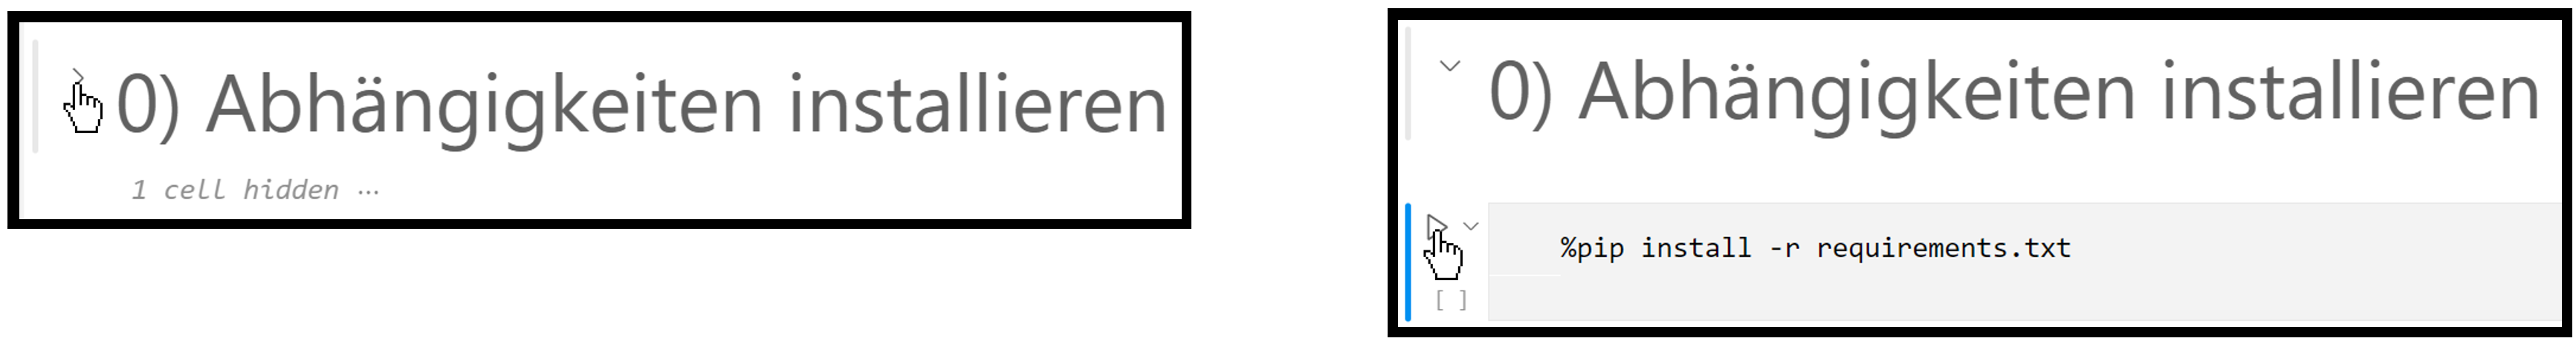
\includegraphics{bilder/cell execution.png}}}
	\caption{Nach Aufklappen der Überschrift eines Ausführungsschritts (links) kann der Python Code in der Zelle ausgeführt werden (rechts).}
\end{figure}

\section*{0) Abhängigkeiten installieren}
Bevor das Python Programm ausgeführt werden kann, müssen alle notwendigen Bibliotheken installiert werden: \textit{Numpy} und \textit{Scipy} unterstützen mathematische Berechnungen während \textit{matplotlib} zur Visualisierung dient. Im Fall der lokalen Ausführung werden mit \texttt{pip install -r requirements.txt} die benötigten Pakete installiert Anschließend muss VSCode und Anaconda Navigator komplett neu gestartet werden. Beim Notebook für Google Colab wird zusätzlich das Repository geklont. Ein Neustart ist dort nicht erforderlich.

\section*{1) Szenario auswählen}
\enlargethispage{1.5cm}
Dieser Ausführungsschritt gruppiert als Ausnahme mehrere Zellen, wobei eine Zelle einem vorkonfiguriertem \textit{Szenario} entspricht. Für ein Szenario müssen alle Parameter des Programms konfiguriert werden, beispielsweise die Dimensionen des Roboters, dessen Start- und Zielposition sowie die Position der Hindernisse. Es werden nur die Parameter der zuletzt ausgeführten Zelle dieses Ausführungsschritts übernommen.
\begin{figure}[H]
	\centering
	\footnotesize
%	\hspace*{-0.085\linewidth}
	\centerline{\resizebox{0.81\linewidth}{!}{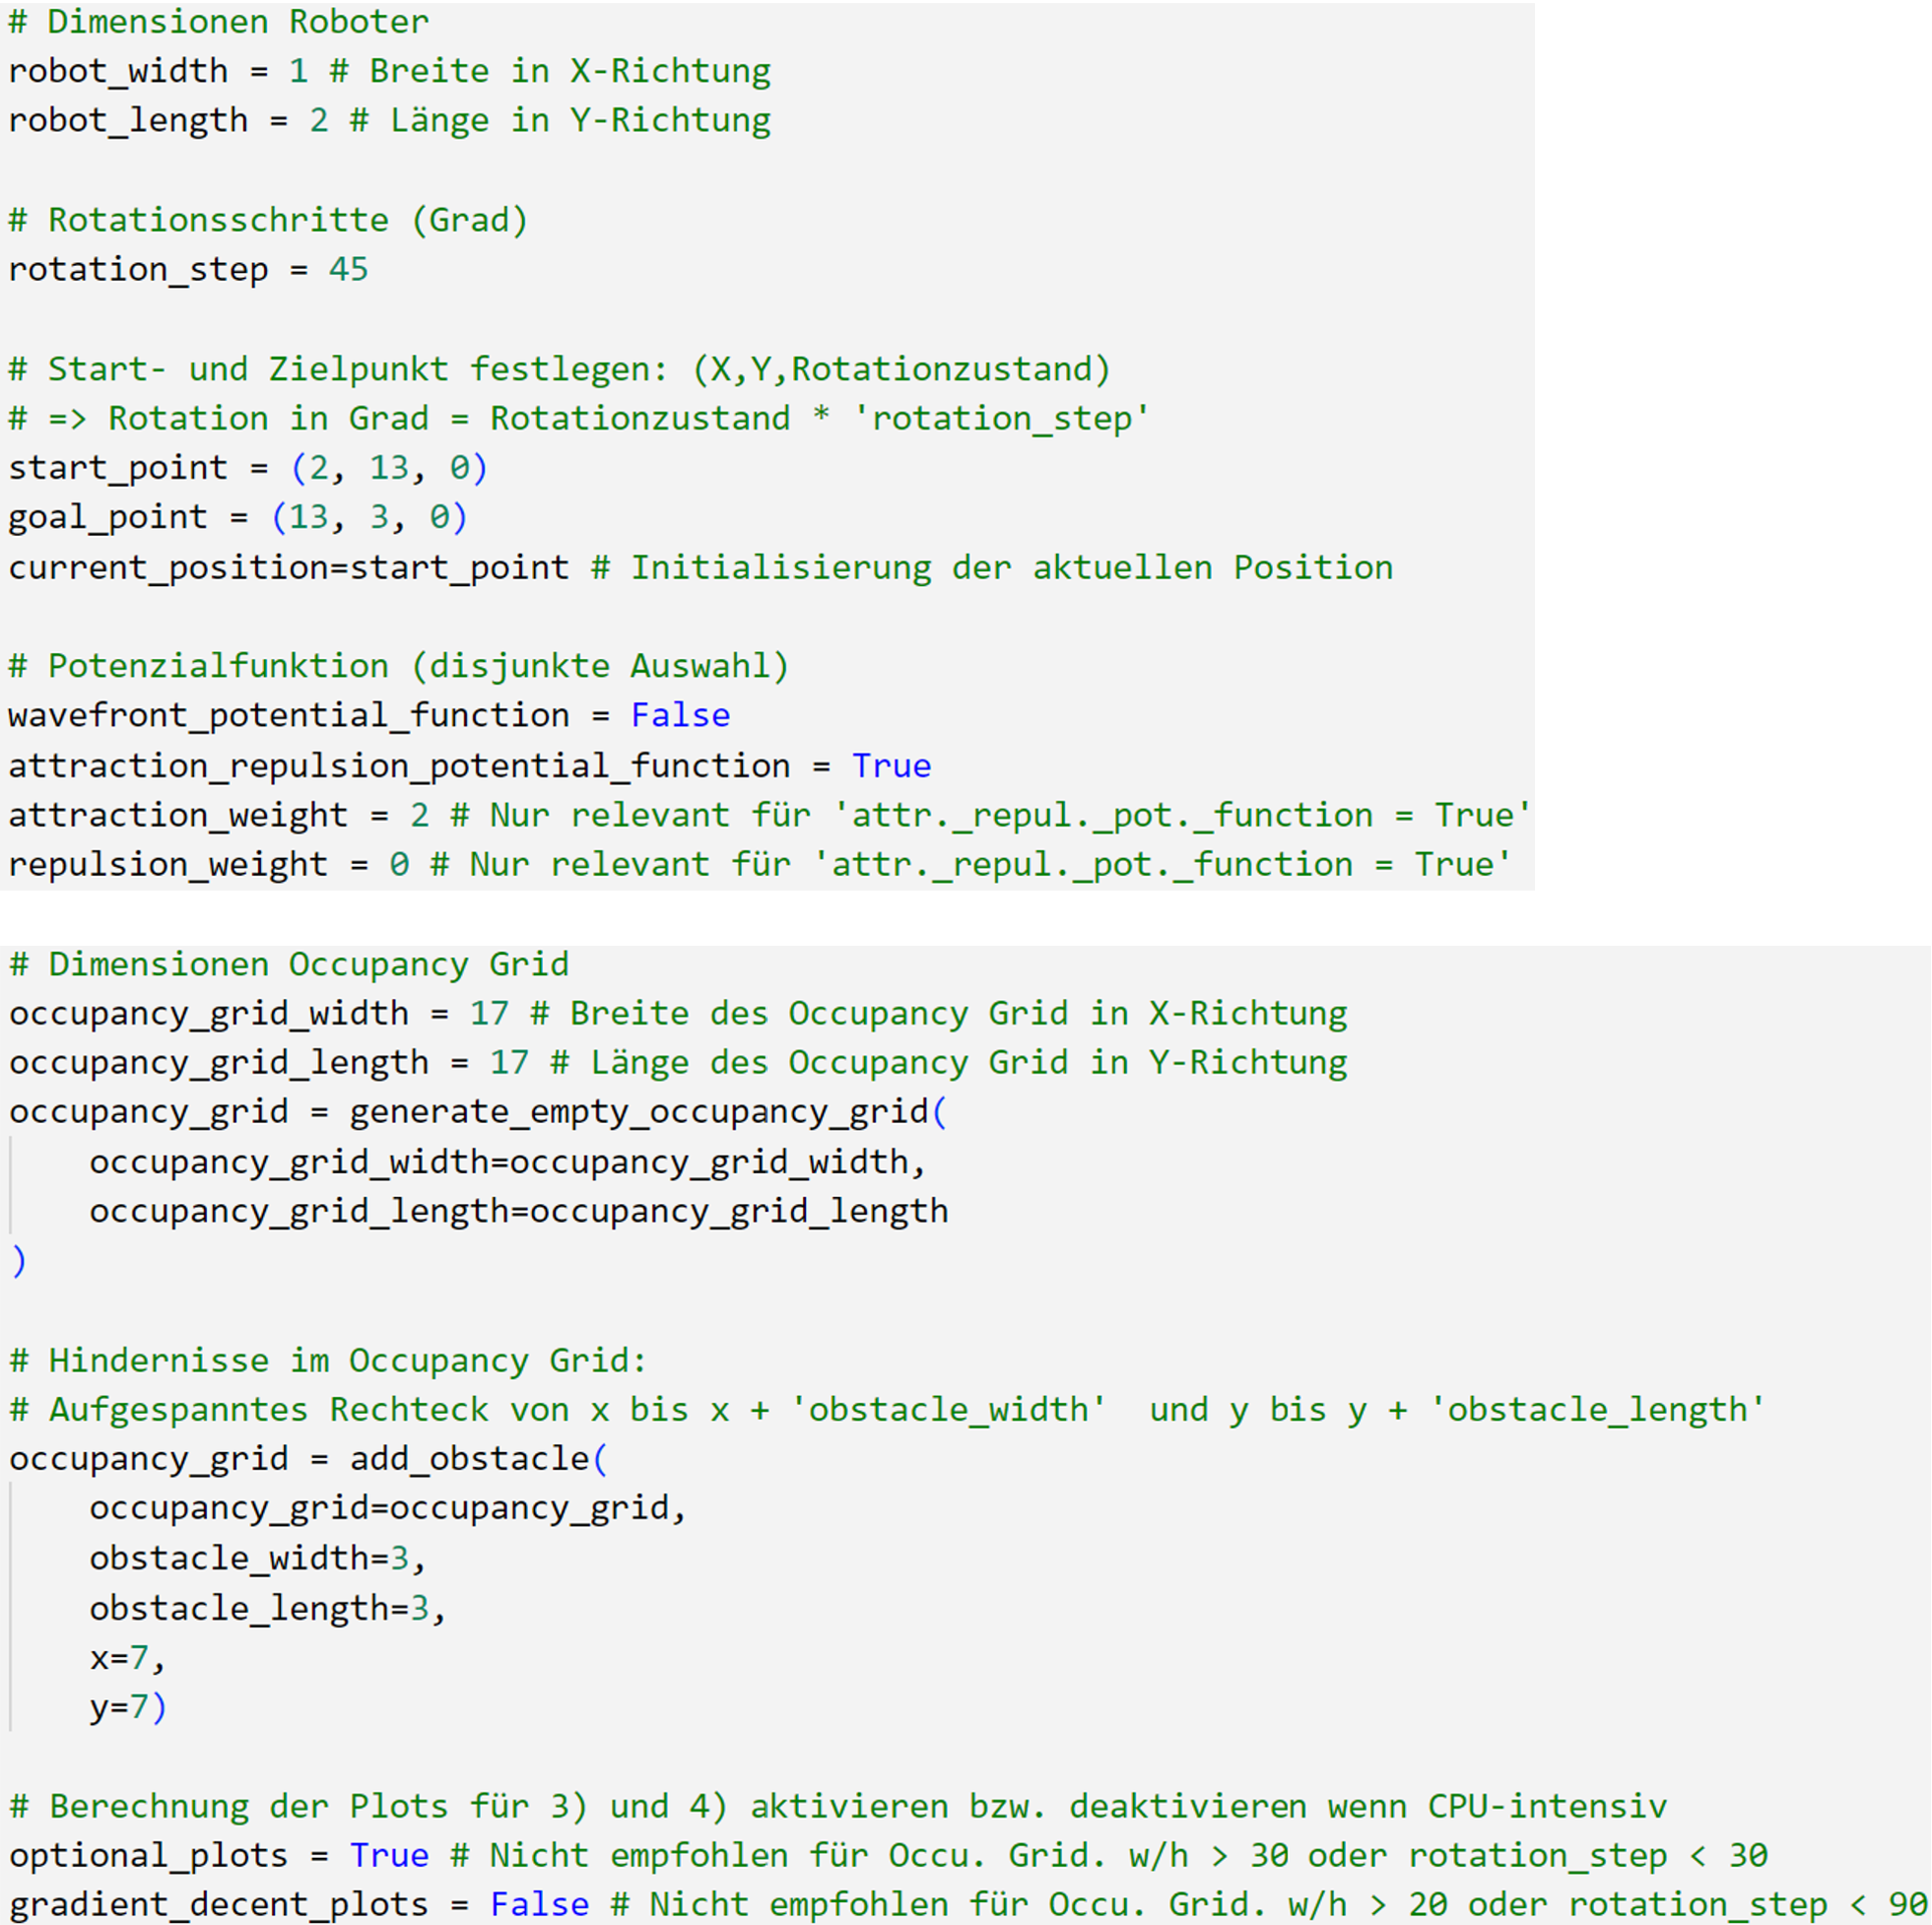
\includegraphics{bilder/parameters2.png}}}
%	\hspace*{-0.115\linewidth}
	\vspace*{-0.2cm}
	\caption{Parameter konfigurieren die gesamte Programmausführung eines Szenarios.}
\end{figure}

\section*{2) Berechnungen durchführen}
In diesem Ausführungsschritt werden die für das Gradientenabstiegsverfahren benötigten mathematischen Berechnungen durchgeführt. Der theoretische Hintergrund der Berechnungen wird in den nachfolgenden Kapitel beschrieben. Änderungen am Python Code dieser Zelle sind nicht notwendig.

\section*{3) Plots ausgeben (optional)}
Als einziger Ausführungsschritt ist die Berechnung und Visualisierung der grafischen Darstellungen optional. Da dieser Schritt sehr rechenaufwändig sein kann, verhindert der im Ausführungsschritts 1) gesetzte Parameter \texttt{optional\_plots=False} bei bestimmten vorkonfigurierten Szenarien die Ausführung dieser Zelle.

\section*{4) Gradientenabstieg initialisieren}
Bedingt durch die matplotlib-Bibliothek muss bei animierten grafischen Darstellungen die Initialisierung von der Ausführungslogik getrennt werden.
Diese Zelle initialisiert ausschließlich das Gradientenabstiegsverfahren und dessen animierte Visualisierung. Wenn im Ausführungsschritt 1) der Parameter \texttt{gradient\_decent\_plots=True} gesetzt wird, werden zusätzliche Plots berechnet. Analog zum Parameter \texttt{optional\_plots=False} des vorherigen Ausführungsschritts wird dies aufgrund des hohen Ressourcenverbrauchs für gewissen Szenarien nicht empfohlen.

\section*{5) Gradientenabstieg starten}
Beim Ausführen dieser Zelle wird das zuvor initialisierte Gradientenabstiegsverfahren gestartet. Im Plot des vorherigen Ausführungsschritts wird die Roboternavigation animiert.
Um ein weiteres Szenario auszuführen, müssen die Ausführungsschritte ab 1) wiederholt werden.


